% =====================================================================
%  IT5425 -- Capstone slide deck
%  Paris 2024 Olympic Data Story (Beamer)
%
%  Engine: tectonic / XeLaTeX.   Build: cd report_and_slides && tectonic presentation.tex
%  Figures: regenerate from repo root with `python scripts/make_figures.py`
%           (written to ../figures/, resolved via \graphicspath below).
% =====================================================================
\documentclass[aspectratio=169,11pt]{beamer}

\usepackage{graphicx}
% This file lives in report_and_slides/; figures are one level up in ../figures/.
\graphicspath{{../}{./}}
\usepackage{tabularx}
\usepackage{booktabs}
\usepackage{helvet}
\renewcommand{\familydefault}{\sfdefault}

% ---- Palette: charcoal / gold / teal / coral -----------------------
\definecolor{charcoal}{HTML}{20242A}
\definecolor{slate}{HTML}{475569}
\definecolor{gold}{HTML}{C8920A}
\definecolor{teal}{HTML}{2A9D8F}
\definecolor{coral}{HTML}{D95F59}
\definecolor{ocean}{HTML}{3A6EA5}
\definecolor{rulegray}{HTML}{D9DEE7}
\definecolor{softgray}{HTML}{F4F6F8}

% ---- Theme (built by hand, no external theme files) ----------------
\usetheme{default}
\useinnertheme{rectangles}
\setbeamertemplate{navigation symbols}{}
\setbeamercolor{normal text}{fg=charcoal}
\setbeamercolor{structure}{fg=teal}
\setbeamercolor{frametitle}{fg=charcoal}
\setbeamercolor{title}{fg=charcoal}
\setbeamercolor{itemize item}{fg=teal}
\setbeamercolor{itemize subitem}{fg=gold}
\setbeamercolor{block title}{fg=white,bg=teal}
\setbeamercolor{block body}{fg=charcoal,bg=softgray}
\setbeamerfont{frametitle}{series=\bfseries,size=\Large}
\setbeamerfont{title}{series=\bfseries,size=\Huge}
\setbeamertemplate{itemize item}{\small\raise0.4pt\hbox{\textbullet}}

% Gold rule + section name under each frame title
\setbeamertemplate{frametitle}{%
  \vspace{8pt}\hspace{6pt}%
  {\usebeamerfont{frametitle}\color{charcoal}\insertframetitle}\\[2pt]
  \hspace{6pt}{\color{gold}\rule{0.45\paperwidth}{1.6pt}}%
}
% Footline: project | section | page
\setbeamertemplate{footline}{%
  \hbox{\begin{beamercolorbox}[wd=\paperwidth,ht=2.6ex,dp=1.2ex,leftskip=8pt,rightskip=8pt]{}%
    \color{slate}\scriptsize Paris 2024 Olympic Data Story
    \hfill \color{slate}\scriptsize IT5425 Capstone
    \hfill \color{slate}\scriptsize \insertframenumber\,/\,\inserttotalframenumber%
  \end{beamercolorbox}}%
}

\newcommand{\teallead}[1]{{\color{teal}\textbf{#1}}}
\newcommand{\techtag}[1]{{\footnotesize\color{gold}\textbf{Technique:} \color{slate}#1}}

% =====================================================================
\begin{document}

% ----------------------------- TITLE --------------------------------
\begin{frame}[plain]
  \vfill
  \begin{center}
    {\small\bfseries\color{charcoal} HANOI UNIVERSITY OF SCIENCE AND TECHNOLOGY}\\[2pt]
    {\footnotesize\color{slate} School of Information and Communications Technology}\\[10pt]
    {\color{gold}\rule{0.86\paperwidth}{2pt}}\\[10pt]
    {\Huge\bfseries\color{charcoal} Paris 2024 Olympic Data Story}\\[8pt]
    {\large\color{teal} A Streamlit dashboard and its visualization techniques}\\[6pt]
    {\color{slate} IT5425 -- Data Management \& Visualization $\cdot$ Capstone demo}\\[8pt]
    {\footnotesize\color{slate} Chu Xuan Minh $\cdot$ Nguyen Binh Anh $\cdot$ Vu Thuy Linh
    $\cdot$ Nguyen Thanh Vinh $\cdot$ Nguyen Dinh Truong}\\[3pt]
    {\footnotesize\color{slate} Supervisor: Tran Viet Trung}\\[10pt]
    {\color{gold}\rule{0.86\paperwidth}{2pt}}\\[14pt]
    {\footnotesize\color{slate} Dataset: official Paris 2024 CSVs (Kaggle) + data.gouv.fr enriched athletes (ODbL)
    $\cdot$ Tool: Streamlit + Plotly}
  \end{center}
  \vfill
\end{frame}

% --------------------------- DATASET --------------------------------
\begin{frame}{The dataset}
  \begin{columns}[T]
    \begin{column}{0.52\textwidth}
      \small
      Public Paris~2024 CSVs (Kaggle ``Paris 2024 Olympic Summer Games'' +
      data.gouv.fr), joined into one working table --- both on Google Dataset
      Search:
      \begin{itemize}
        \item \teallead{11,113} athletes across \teallead{206} NOCs
        \item \teallead{45} disciplines, \teallead{2,268} athlete--medal records
        \item Enriched athletes: age, venue coordinates, dates, record flag
        \item \teallead{41} venues with valid coordinates
      \end{itemize}
    \end{column}
    \begin{column}{0.46\textwidth}
      \centering
      \vspace{-6pt}
      \begin{block}{Two distinct medal concepts}
        \footnotesize
        \textbf{Country totals} count official medals by NOC.\\[3pt]
        \textbf{Athlete--medal records} count each athlete on a medal, so team
        sports multiply.\\[3pt]
        The dashboard keeps them on separate pages and labels the unit.
      \end{block}
      \vspace{6pt}
      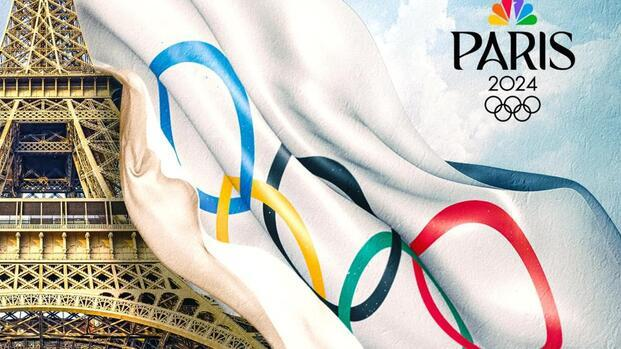
\includegraphics[width=0.88\linewidth]{assets/olympic-2024-2.jpg}
    \end{column}
  \end{columns}
\end{frame}

% --------------------------- OBJECTIVE ------------------------------
\begin{frame}{Objective and story arc}
  \small
  \textbf{Problem.} A flat medal table hides geography, specialization,
  demographics, and venue spread.\\[4pt]
  \textbf{Goal.} Four sections, broad to narrow: follow the \teallead{guided
  story} first, then use the \teallead{filters} to explore on each page.
  \vspace{6pt}
  \begin{columns}[T]
    \column{0.24\textwidth}\centering
      {\color{gold}\textbf{1}}\\ \footnotesize Opening Lens\\ \scriptsize\color{slate} global scale, geography \& venues
    \column{0.24\textwidth}\centering
      {\color{gold}\textbf{2}}\\ \footnotesize Medal Race\\ \scriptsize\color{slate} led \& moved vs Tokyo
    \column{0.24\textwidth}\centering
      {\color{gold}\textbf{3}}\\ \footnotesize Specialization\\ \scriptsize\color{slate} NOC $\times$ discipline
    \column{0.24\textwidth}\centering
      {\color{gold}\textbf{4}}\\ \footnotesize Athlete Lens\\ \scriptsize\color{slate} age, gender, load, records
  \end{columns}
  \vspace{8pt}
  \begin{block}{Headline}
    \footnotesize USA and China \textbf{tied at 40 golds} (USA led totals 126--91);
    host \textbf{France +31} vs Tokyo, \textbf{Japan $-13$};
    \textbf{49.1\%} female; median age \textbf{26}; \textbf{64} records.
  \end{block}
\end{frame}

% --------------------------- TECHNIQUE MAP --------------------------
\begin{frame}{Which technique each chart applies}
  \footnotesize
  \renewcommand{\arraystretch}{1.3}
  \begin{tabularx}{\textwidth}{@{}l X@{}}
    \toprule
    {\color{teal}\textbf{Chart}} & {\color{teal}\textbf{Technique demonstrated}} \\
    \midrule
    World choropleth        & Map intensity; nominal$\rightarrow$region, quantitative$\rightarrow$colour \\
    Stacked / diverging bars& Length for amounts; diverging bar for change \\
    Bubble scatter          & Relationship; position + area + hue; overlap control \\
    Country$\times$discipline heatmap & Pre-attentive detection + exact cell values \\
    Medal-flow Sankey       & Bipartite graph (NOC$\rightarrow$discipline); ribbon width = flow \\
    Treemap                 & Hierarchy with proportional ink \\
    Histogram / box plots   & Distributions and spread \\
    Venue symbol map        & Point map; size + colour on coordinates \\
    Daily medal timeline    & Trend over time; animated cumulative race \\
    Inline controls         & Filtering, view transform, \emph{animation}, details-on-demand \\
    \bottomrule
  \end{tabularx}
\end{frame}

% --------------------------- VIZ 1: MAP -----------------------------
\begin{frame}{Opening Lens --- global medal geography}
  \begin{columns}[c]
    \column{0.62\textwidth}\centering
      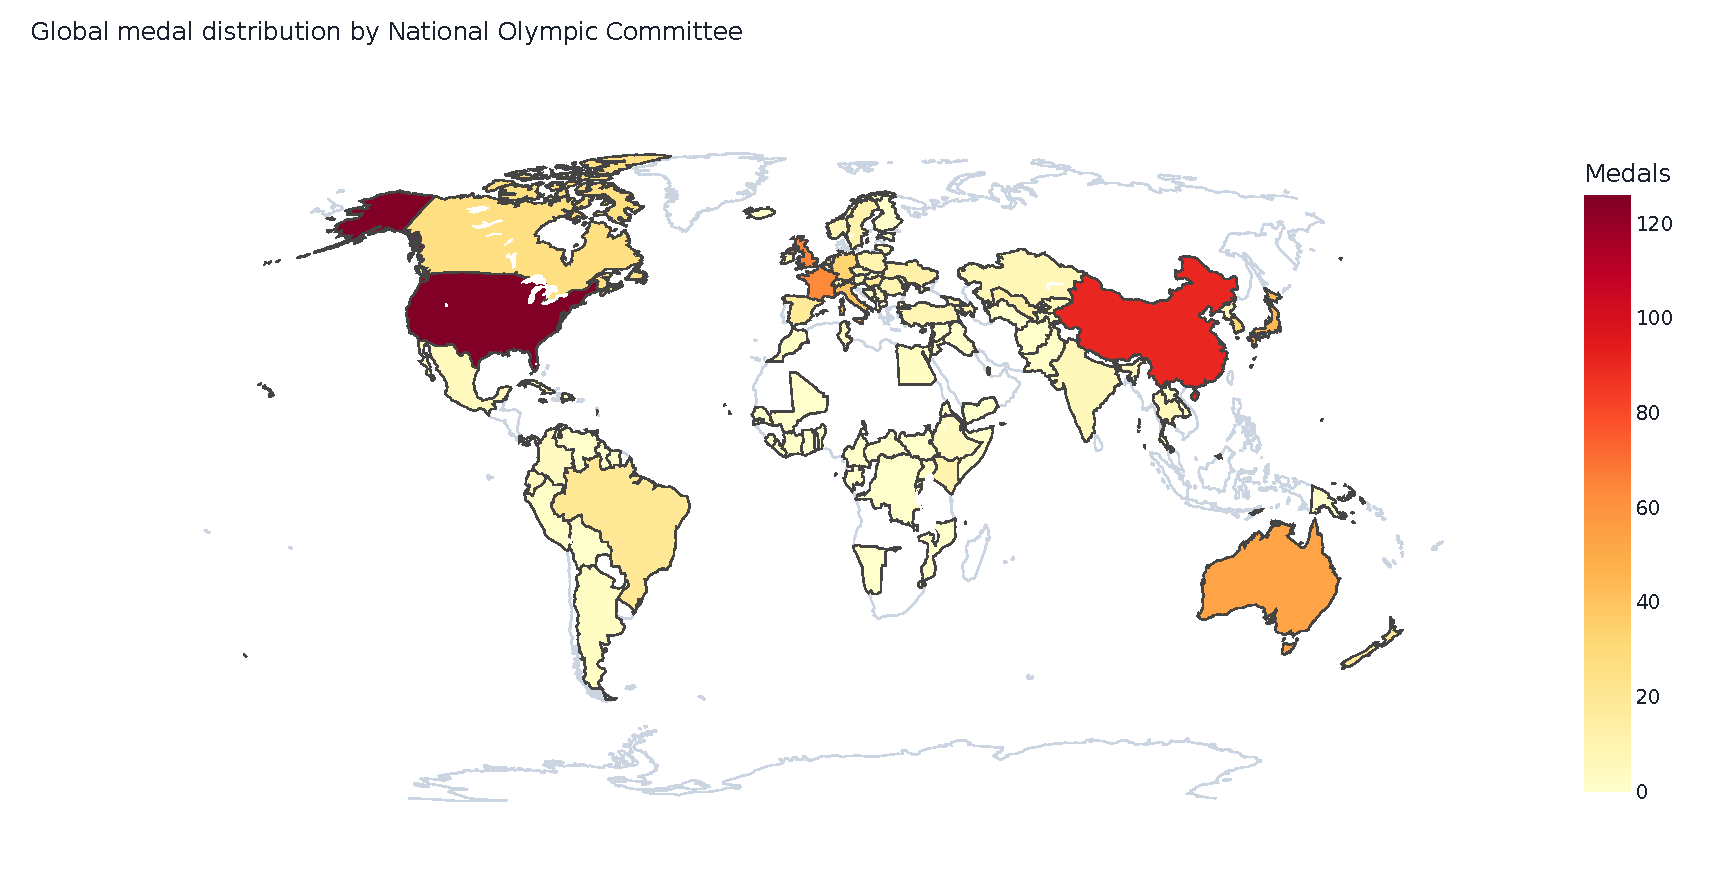
\includegraphics[width=\linewidth]{figures/world_medal_map.pdf}
    \column{0.36\textwidth}\small
      Colour intensity makes the USA--China lead \teallead{visible before you
      read a single label}. NOC codes are mapped to ISO-3 so country geometry
      works.\\[6pt]
      \techtag{Choropleth; colour-intensity encoding; pre-attentive processing.}
  \end{columns}
\end{frame}

% --------------------------- VIZ 2: HEATMAP -------------------------
\begin{frame}{Sport Specialization --- who wins what}
  \begin{columns}[c]
    \column{0.66\textwidth}\centering
      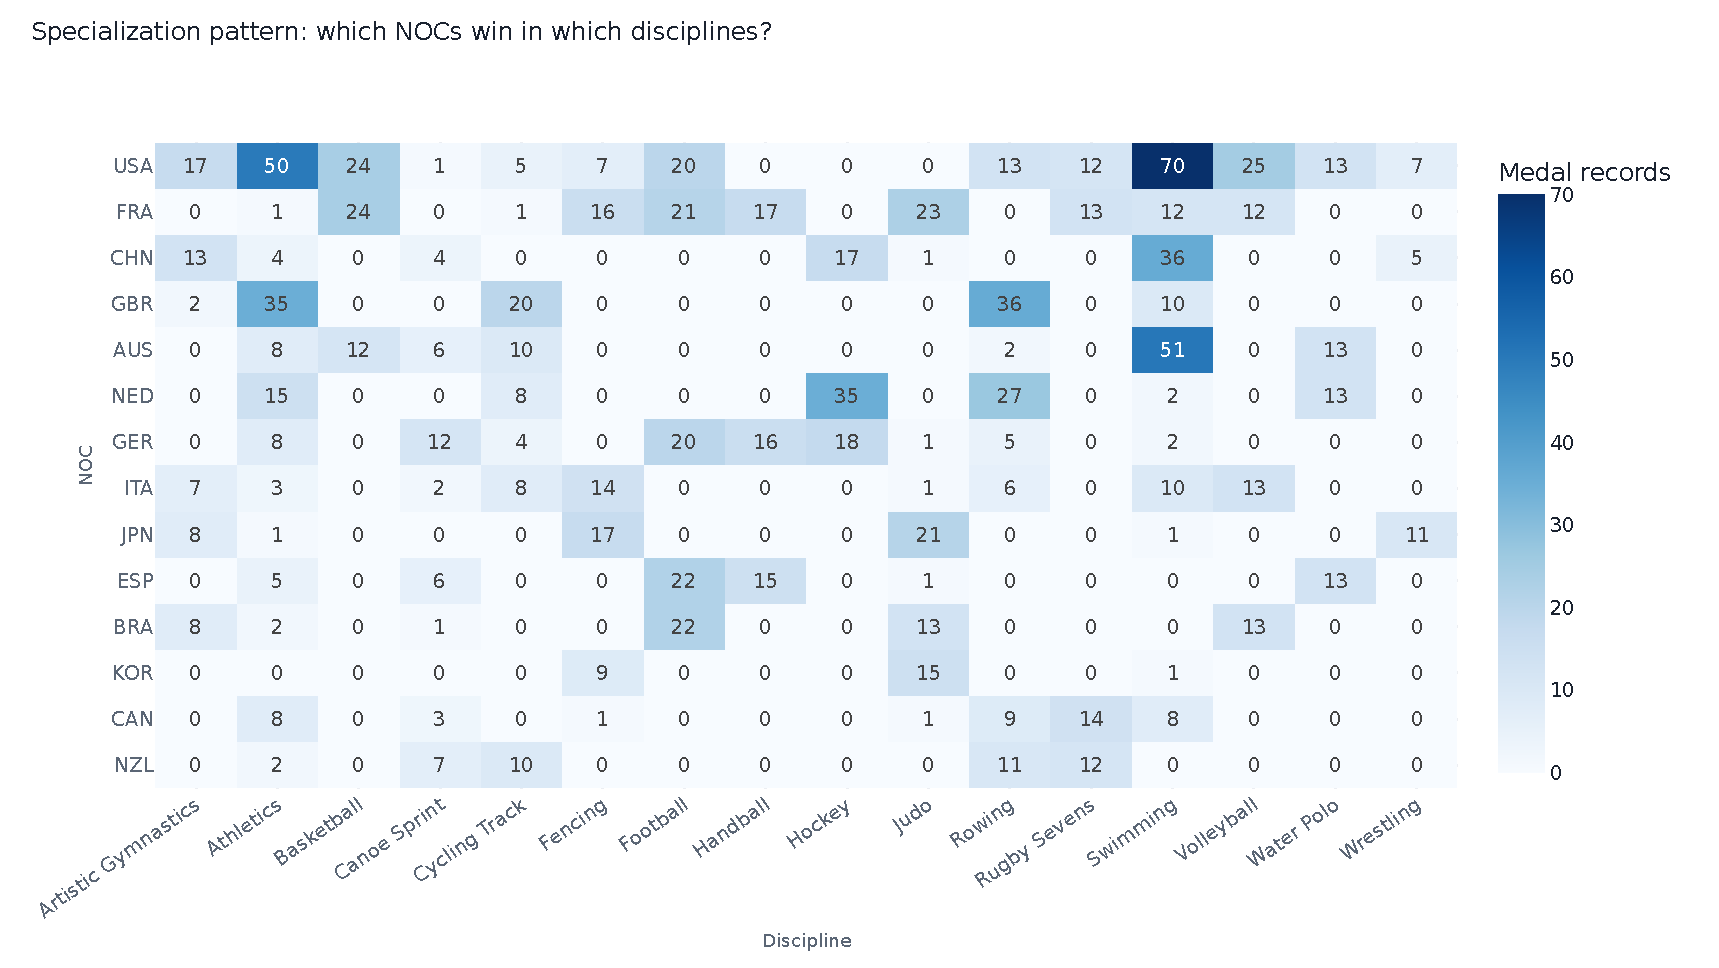
\includegraphics[width=\linewidth]{figures/specialization_heatmap.pdf}
    \column{0.32\textwidth}\small
      Dark cells (USA swimming~=70, NED hockey, GBR rowing) are spotted
      instantly; \teallead{printed values} give exact magnitudes where colour is
      imprecise.\\[6pt]
      \techtag{Pre-attentive detection + multiple encodings.}
  \end{columns}
\end{frame}

% --------------------------- VIZ 3: SANKEY --------------------------
\begin{frame}{A derived flow graph}
  \begin{columns}[c]
    \column{0.64\textwidth}\centering
      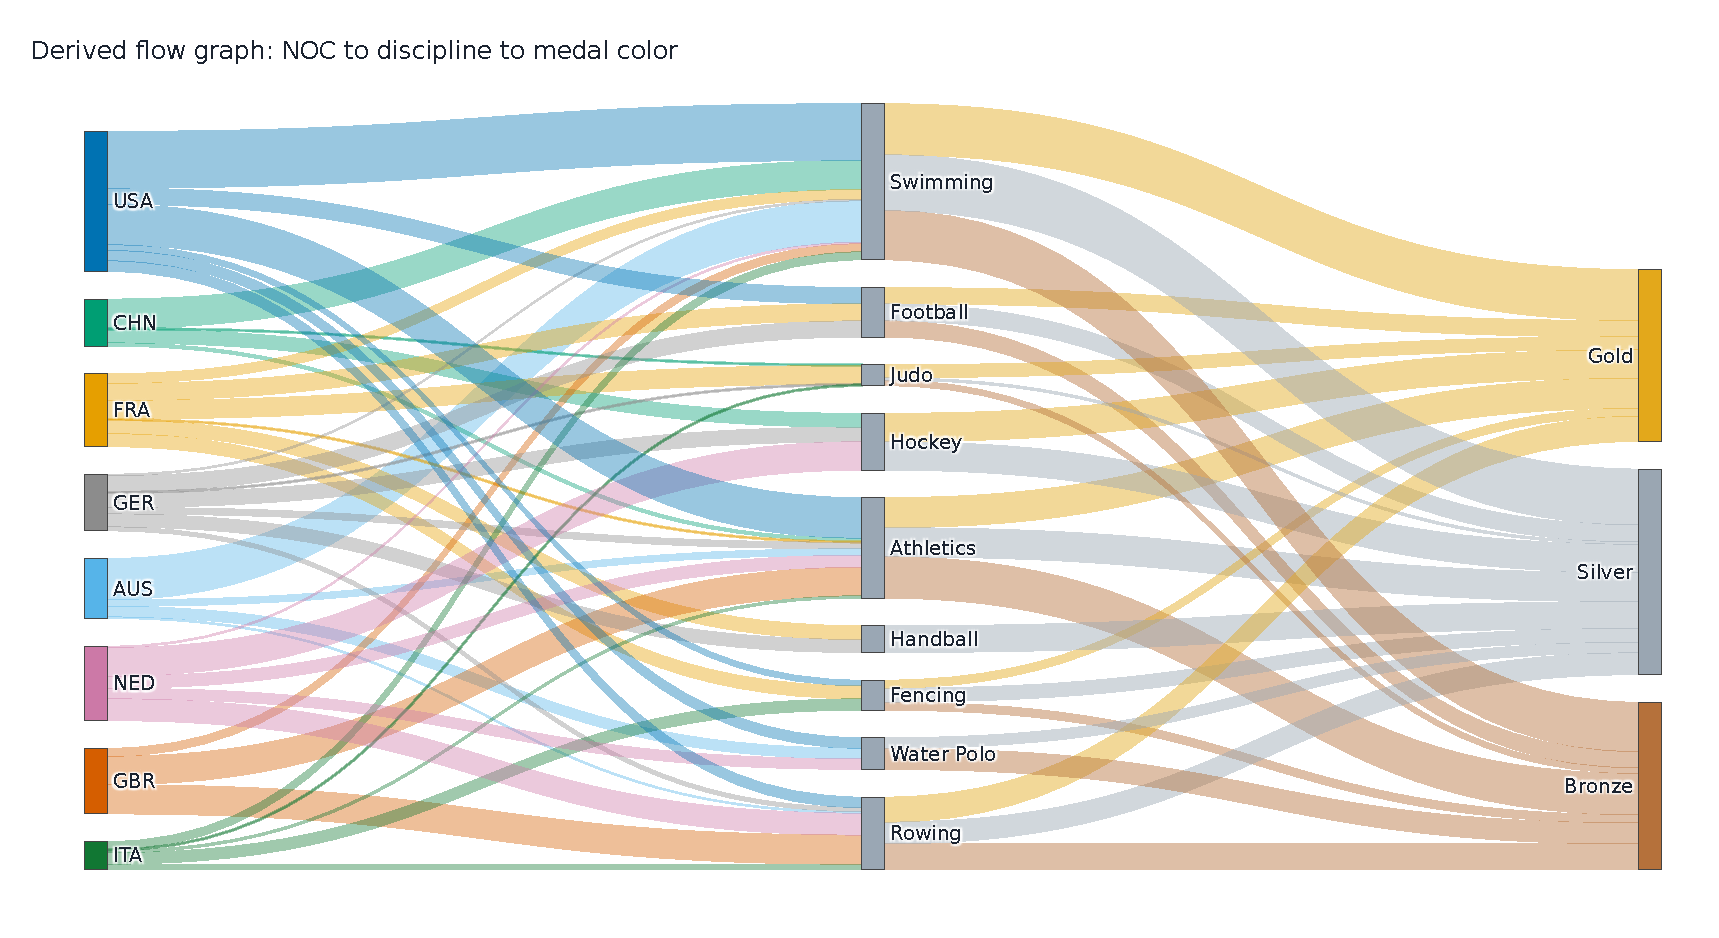
\includegraphics[width=\linewidth]{figures/medal_flow_sankey.pdf}
    \column{0.34\textwidth}\small
      A \teallead{bipartite} flow, NOC~$\rightarrow$~discipline, with
      \teallead{ribbon width = record volume}. The widest ribbons mark the
      strongest nation--sport pairings.\\[6pt]
      \techtag{Graph visualization (Sankey mechanism).}
  \end{columns}
\end{frame}

% --------------------------- VIZ 3b: MEDAL TIMELINE -----------------
\begin{frame}{The medal race over time --- and the one animation}
  \begin{columns}[c]
    \column{0.64\textwidth}\centering
      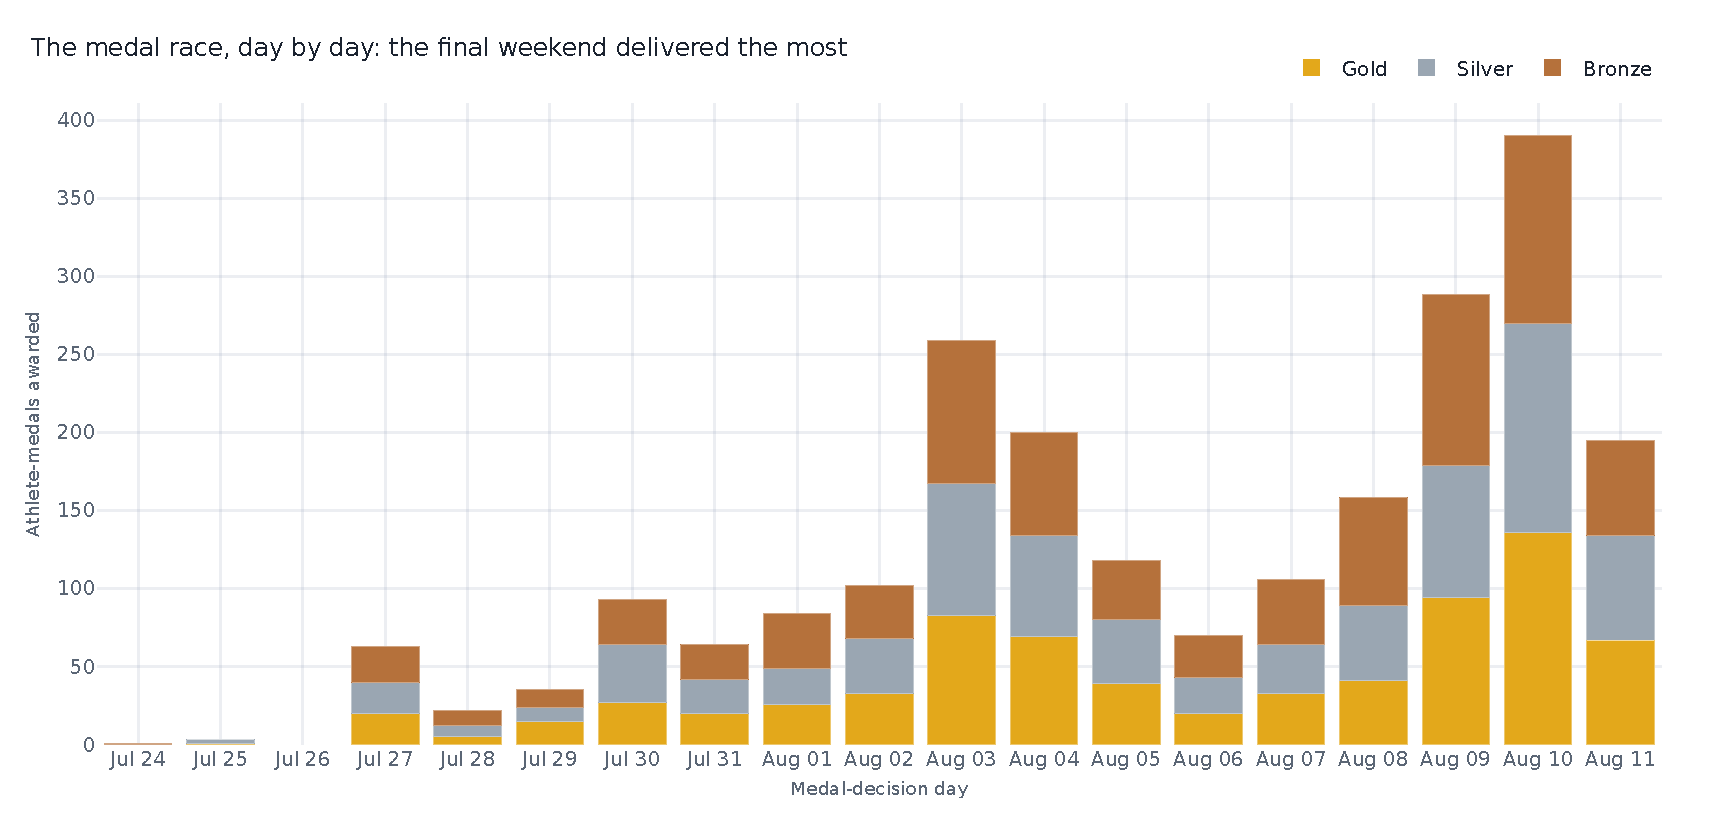
\includegraphics[width=\linewidth]{figures/daily_medals.pdf}
    \column{0.34\textwidth}\small
      Athlete-medals by Games day: the tally \teallead{surges on the closing
      weekend}. A Daily\,/\,Cumulative toggle and an \teallead{animated bar-chart
      race} (press play) add the time dimension.\\[6pt]
      \techtag{Trend over time; animation (used only where the
      variable is time-ordered).}
  \end{columns}
\end{frame}

% --------------------------- VIZ 4: DISTRIBUTIONS -------------------
\begin{frame}{Athlete Lens --- distributions and proportions}
  \begin{columns}[c]
    \column{0.5\textwidth}\centering
      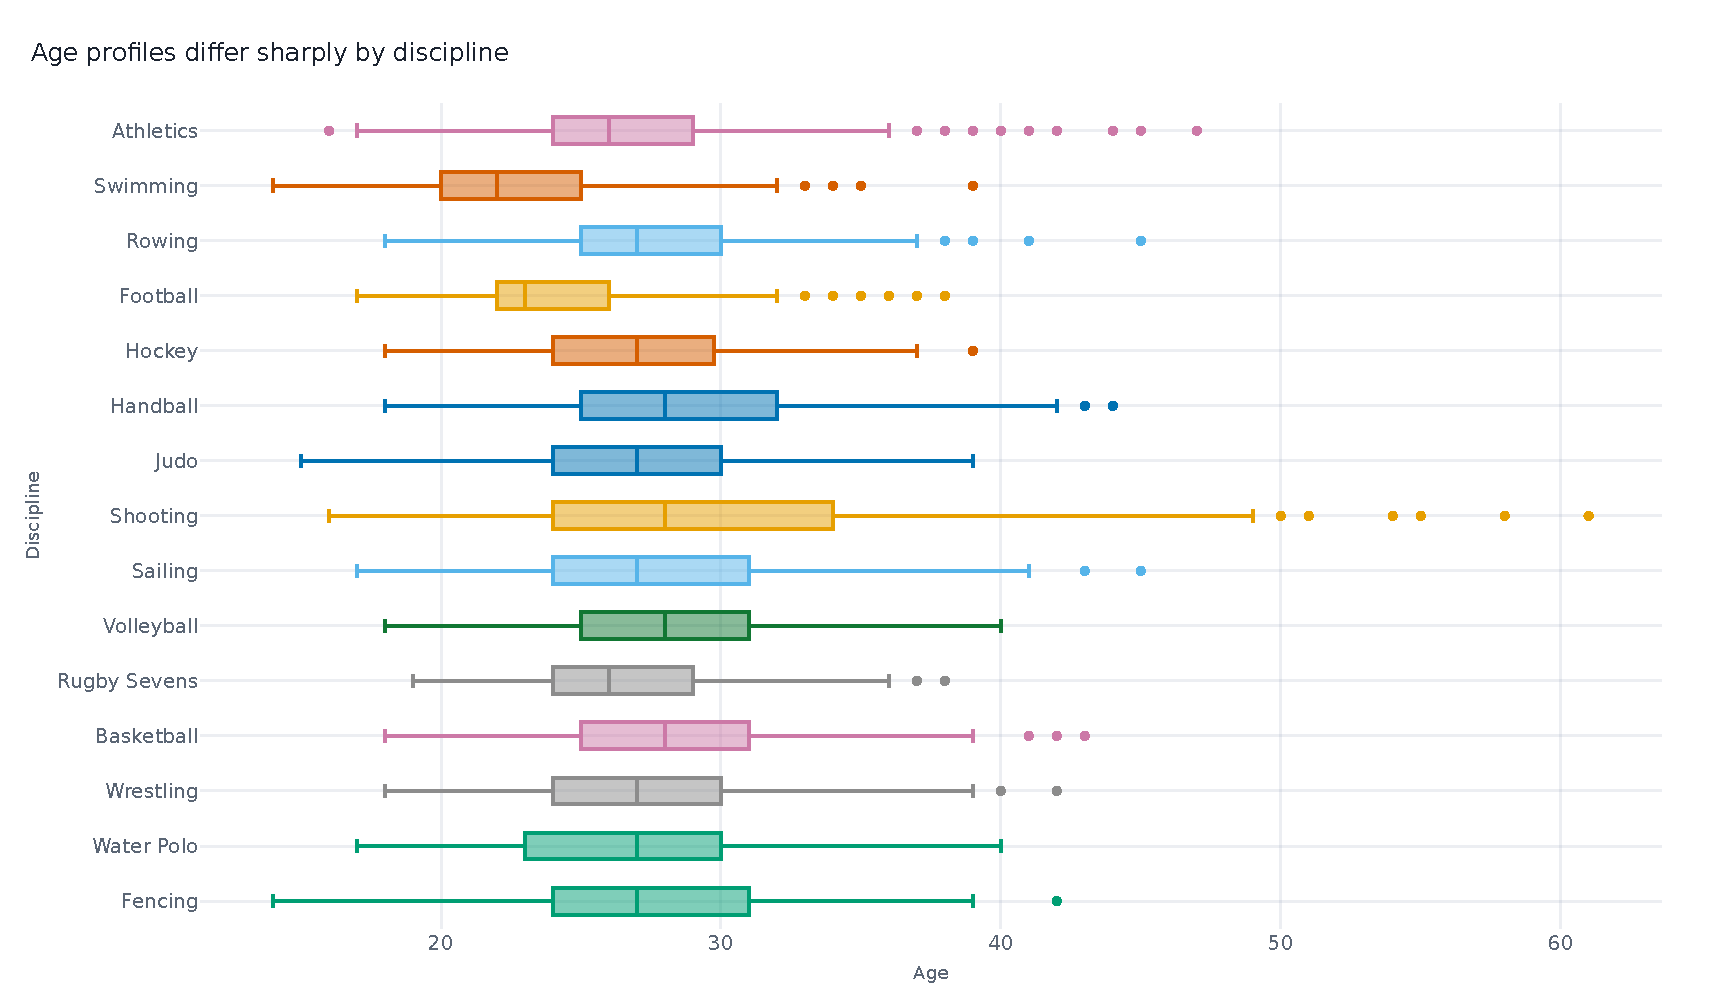
\includegraphics[width=\linewidth]{figures/age_by_discipline.pdf}
    \column{0.5\textwidth}\centering
      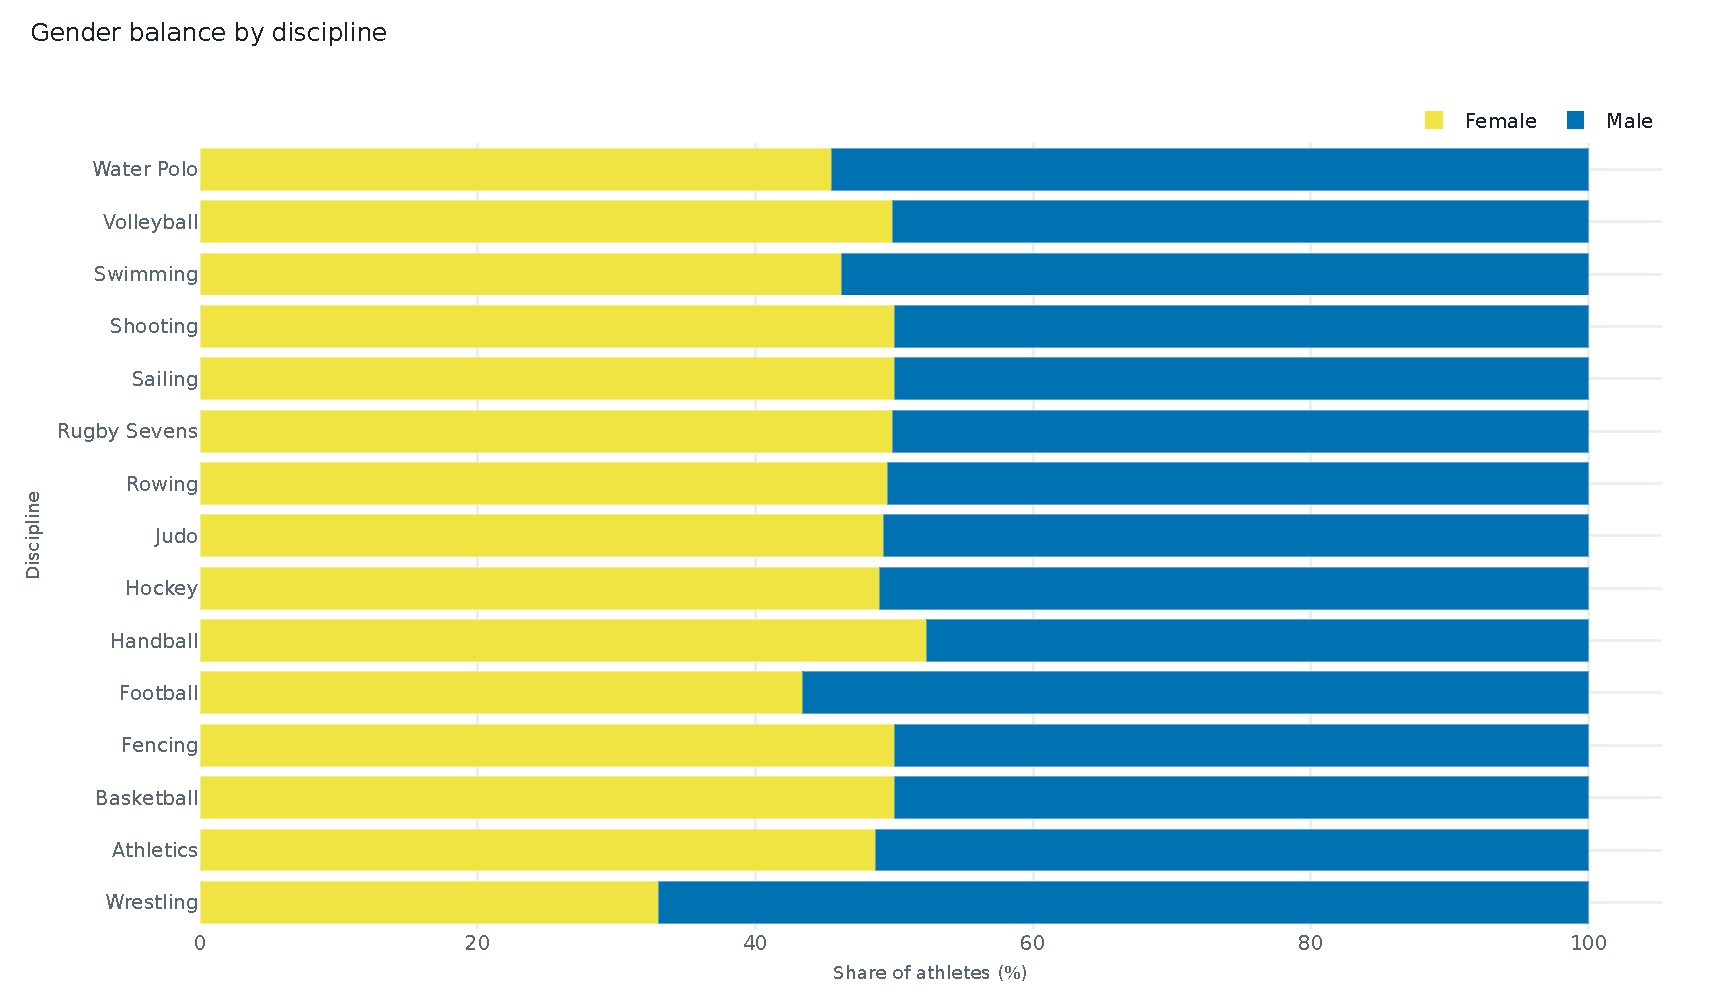
\includegraphics[width=\linewidth]{figures/gender_balance.pdf}
  \end{columns}
  \vspace{2pt}
  \centering\small
  Age medians span \teallead{20} (skateboarding) to \teallead{39} (equestrian);
  near gender parity at \teallead{49.1\%} female.\quad
  \techtag{Distributions (box) \& proportions (100\% stacked).}
\end{frame}

% --------------------------- VIZ 5: CHANGE --------------------------
\begin{frame}{Medal Race --- who moved most since Tokyo}
  \begin{columns}[c]
    \column{0.6\textwidth}\centering
      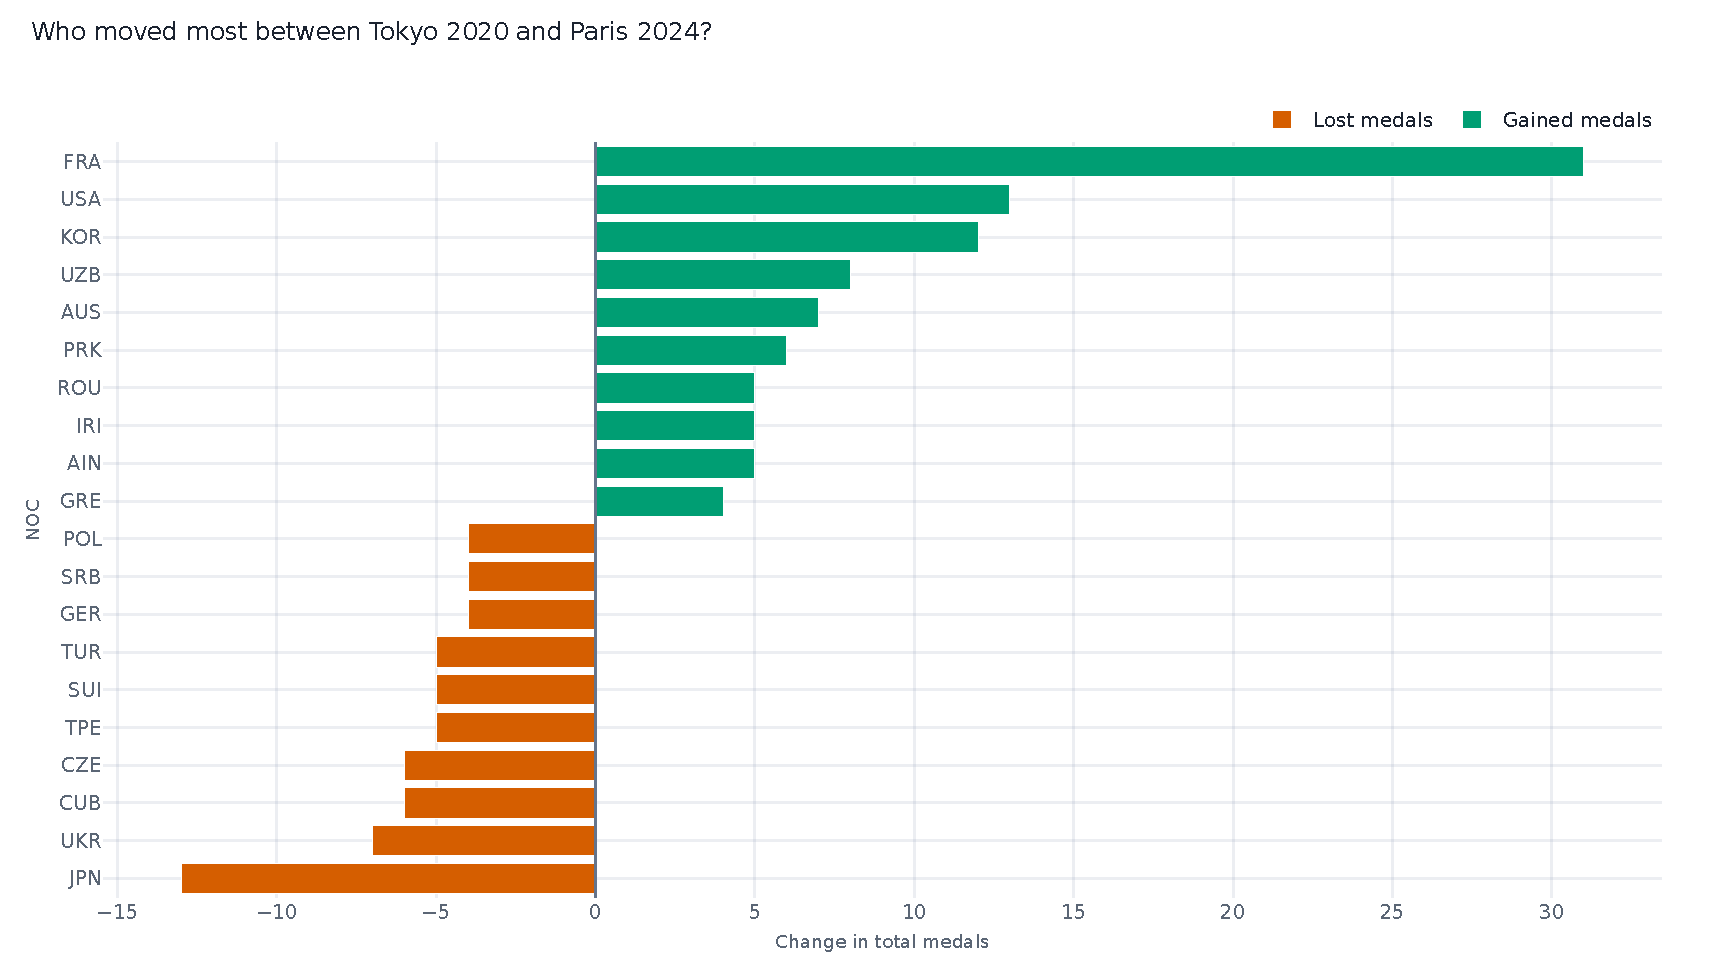
\includegraphics[width=\linewidth]{figures/tokyo_delta.pdf}
    \column{0.38\textwidth}\small
      A \teallead{diverging bar} around zero: host \textbf{France +31}, while
      \textbf{Japan $-13$}. Direction is labelled so colour is never the only
      cue.\\[6pt]
      \techtag{Visualizing change; accessible colour.}
  \end{columns}
\end{frame}

% --------------------------- VIZ 6: VENUE MAP -----------------------
\begin{frame}{Opening Lens --- the spatial footprint}
  \begin{columns}[c]
    \column{0.62\textwidth}\centering
      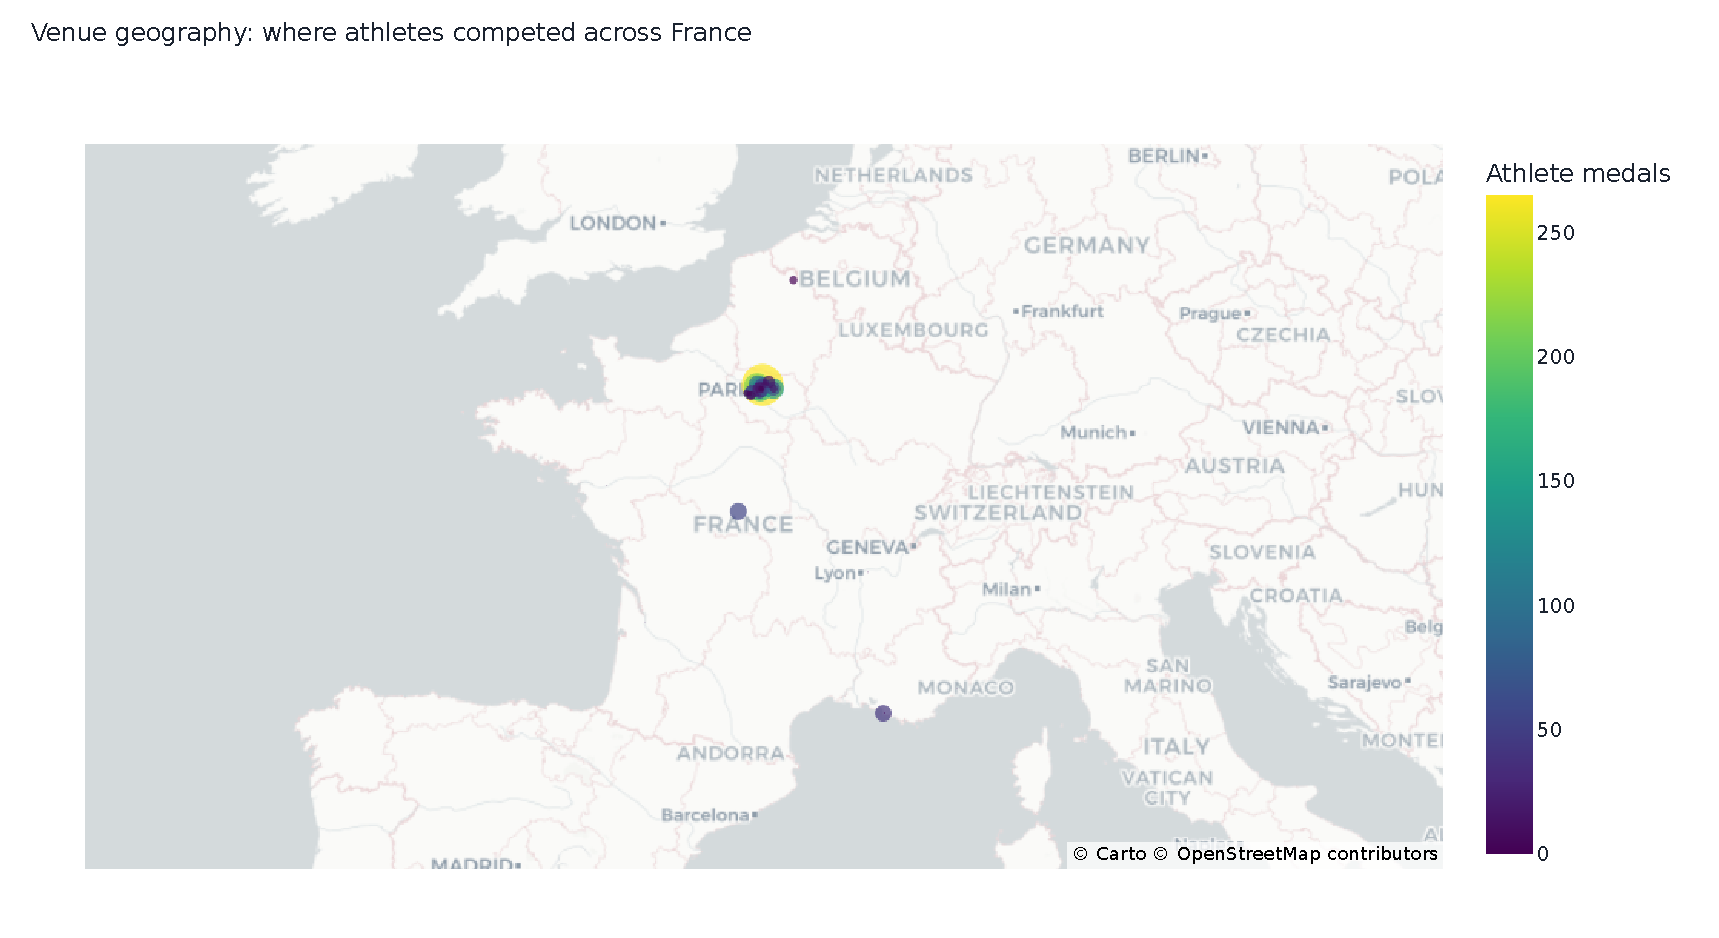
\includegraphics[width=\linewidth]{figures/venue_geography.pdf}
    \column{0.36\textwidth}\small
      A \teallead{symbol map} closing the Opening Lens: bubble size = athlete
      volume, colour = medal activity. The dense Paris cluster contrasts with
      sailing/surf venues far to the south.\\[6pt]
      \techtag{Point map on lat/long coordinates.}
  \end{columns}
\end{frame}

% --------------------------- INTERACTION ----------------------------
\begin{frame}{Interaction and storytelling}
  \small
  \begin{columns}[T]
    \column{0.5\textwidth}
      \teallead{Interaction}
      \begin{itemize}
        \item Tabs switch sections; every control sits beside the chart it drives
        \item Inline segmented pills + multiselects + sliders
        \item Details-on-demand: hover tooltips; zoom/pan on every chart
        \item Empty filters fall back to styled placeholders, never crash
      \end{itemize}
    \column{0.5\textwidth}
      \teallead{Storytelling}
      \begin{itemize}
        \item We set the story order; viewers use filters on each page
        \item Each section opens with \textbf{summary numbers}, then shows them visually
        \item \textbf{No raw data dumps} --- show the data, detail on hover
        \item Colourblind-safe Okabe--Ito palette; host-nation spotlight
      \end{itemize}
  \end{columns}
  \vspace{4pt}
  \begin{block}{Where we drew the line}
    \footnotesize \textbf{Animation \emph{is} used} --- but only on the medal
    race timeline, where time ordering makes it meaningful. No trend lines or
    error bands: the data is final, nothing is uncertain.
  \end{block}
\end{frame}

% --------------------------- INSIGHTS -------------------------------
\begin{frame}{Key insights}
  \small
  \begin{enumerate}
    \item \teallead{Gold was a dead heat, totals were not.} USA \& China each 40
      gold; USA led on total medals 126--91.
    \item \teallead{Hosting moved the table.} France +31 vs Tokyo (largest swing);
      Japan $-13$.
    \item \teallead{Specialization defines mid-tier powers.} NED hockey, GBR
      rowing, AUS swimming --- concentrated, not broad.
    \item \teallead{Near gender parity, sport-specific ages.} 49.1\% female;
      medians from 20 to 39 by discipline.
    \item \teallead{A dispersed Games.} Venues reach from Paris to Marseille
      sailing and overseas surfing.
  \end{enumerate}
\end{frame}

% --------------------------- CLOSE ----------------------------------
{
\setbeamertemplate{background}{%
  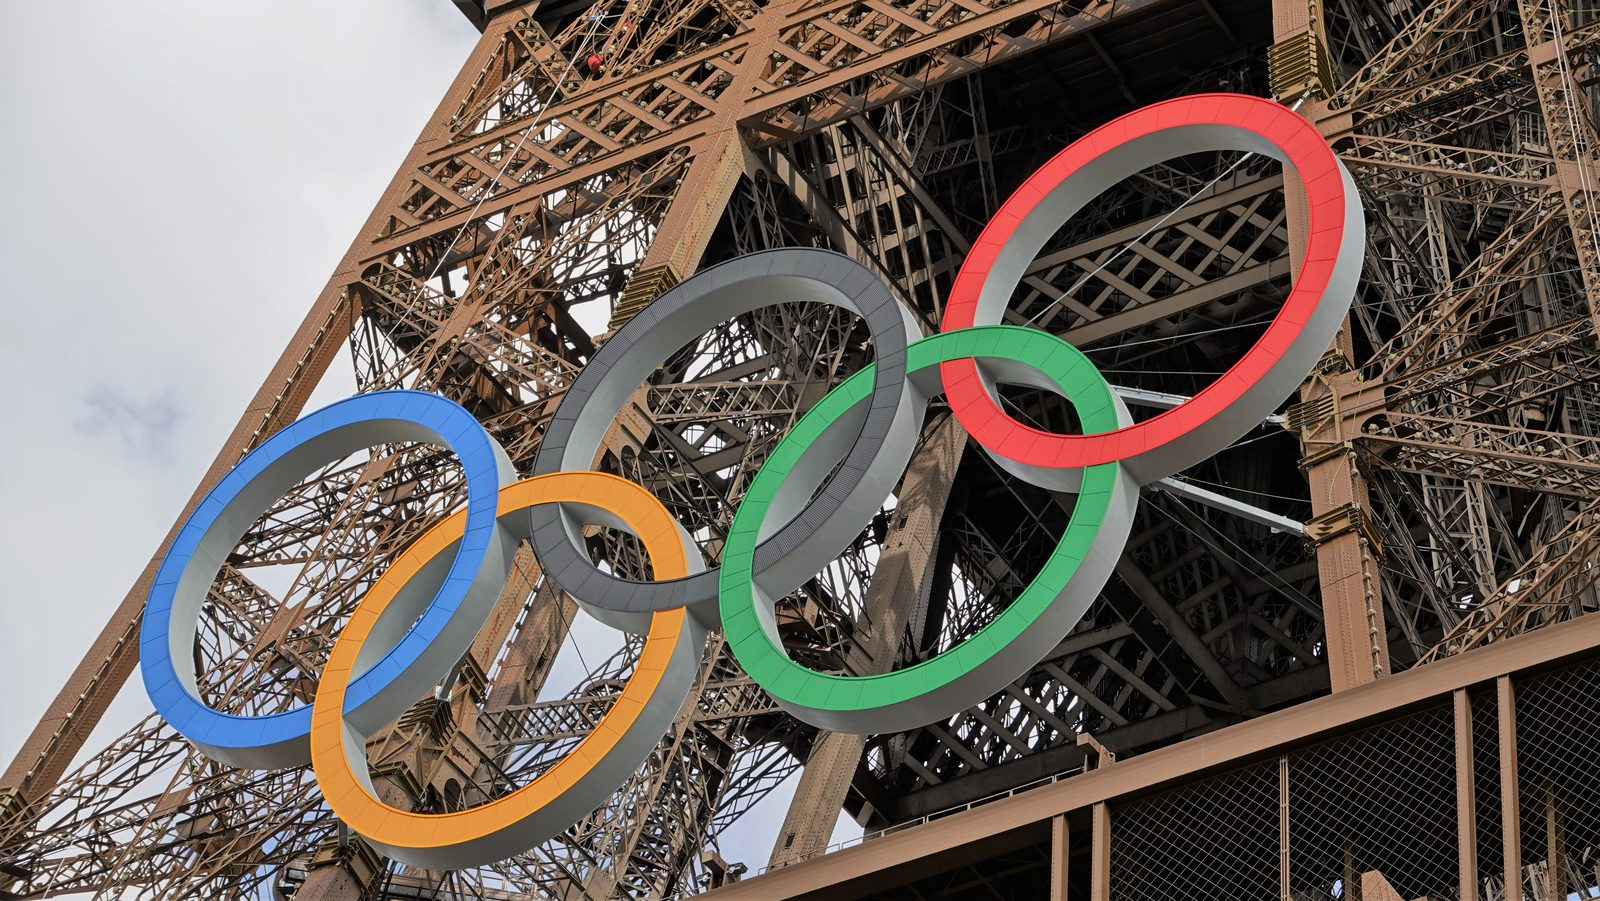
\includegraphics[width=\paperwidth,height=\paperheight]{assets/paris2024_eiffel.jpg}}
\begin{frame}[plain]
  \vfill
  \begin{center}
  \colorbox{charcoal!90}{%
    \begin{minipage}{0.82\paperwidth}\centering\vspace{5pt}
      {\Large\bfseries\color{white} The medal table only tells you who won.}\\[7pt]
      {\color{white!92} Who rose, who specialised, who actually showed up, and where ---\\
      that story only comes out when you can interact with the data.}\\[13pt]
      {\large\bfseries\color{gold} Thank you.}\quad{\color{white!88} We'd love your questions.}
      \vspace{5pt}
    \end{minipage}}
  \end{center}
  \vfill
  \hfill{\tiny\color{white!85} Olympic rings on the Eiffel Tower $\cdot$ photo by Ibex73, CC BY 4.0, via Wikimedia Commons}\hspace{8pt}\strut
\end{frame}
}

\end{document}
